\chapter[Proposta]{Proposta}
O objetivo deste capítulo é apresentar uma possível proposta de solução, a qual deve atender às necessidades colocadas no primeiro capítulo referente à problemática deste trabalho. A apresentação da proposta está concentrada em duas partes. A primeira parte está relacionada à coleta das métricas utilizando a ferramenta SonarQube, e a segunda parte está relacionada à criação do \textit{dashboard} e à visualização das informações. Para analise da presente proposta, foram escolhidos dois projetos, sendo ambos os projetos de código aberto extraídos do portal do software público brasileiro. A terceira e última parte do trabalho consiste em analisar os resultados obtidos através de uma avaliação qualitativa com possíveis usuários.

\section{Ambiente Simulado}
Para se simular um ambiente de produção, será utilizado como modelo de referência o ambiente apresentado por Luiza e Yago \cite{luiza_yago}. No trabalho descrito, os autores caracterizam o órgão pertencente à APF como Órgão X. Uma das características referentes ao Órgão X que podem ser citadas diz respeito a sua área de jurisdição que abrange serviços de radiodifusão, postais e de telecomunicações. O Órgão X atualmente implanta o GeDDAS (Gestão de Demandas de Desenvolvimento Ágil de Software) proposto por Souza \cite{ouza_sobrinho_uso_2014}. A Figura \ref{img:proc_des} apresenta o processo de desenvolvimento adotado pelo Órgão X.

\graphicspath{{figuras/}}
\begin{figure}[h!]
\centering
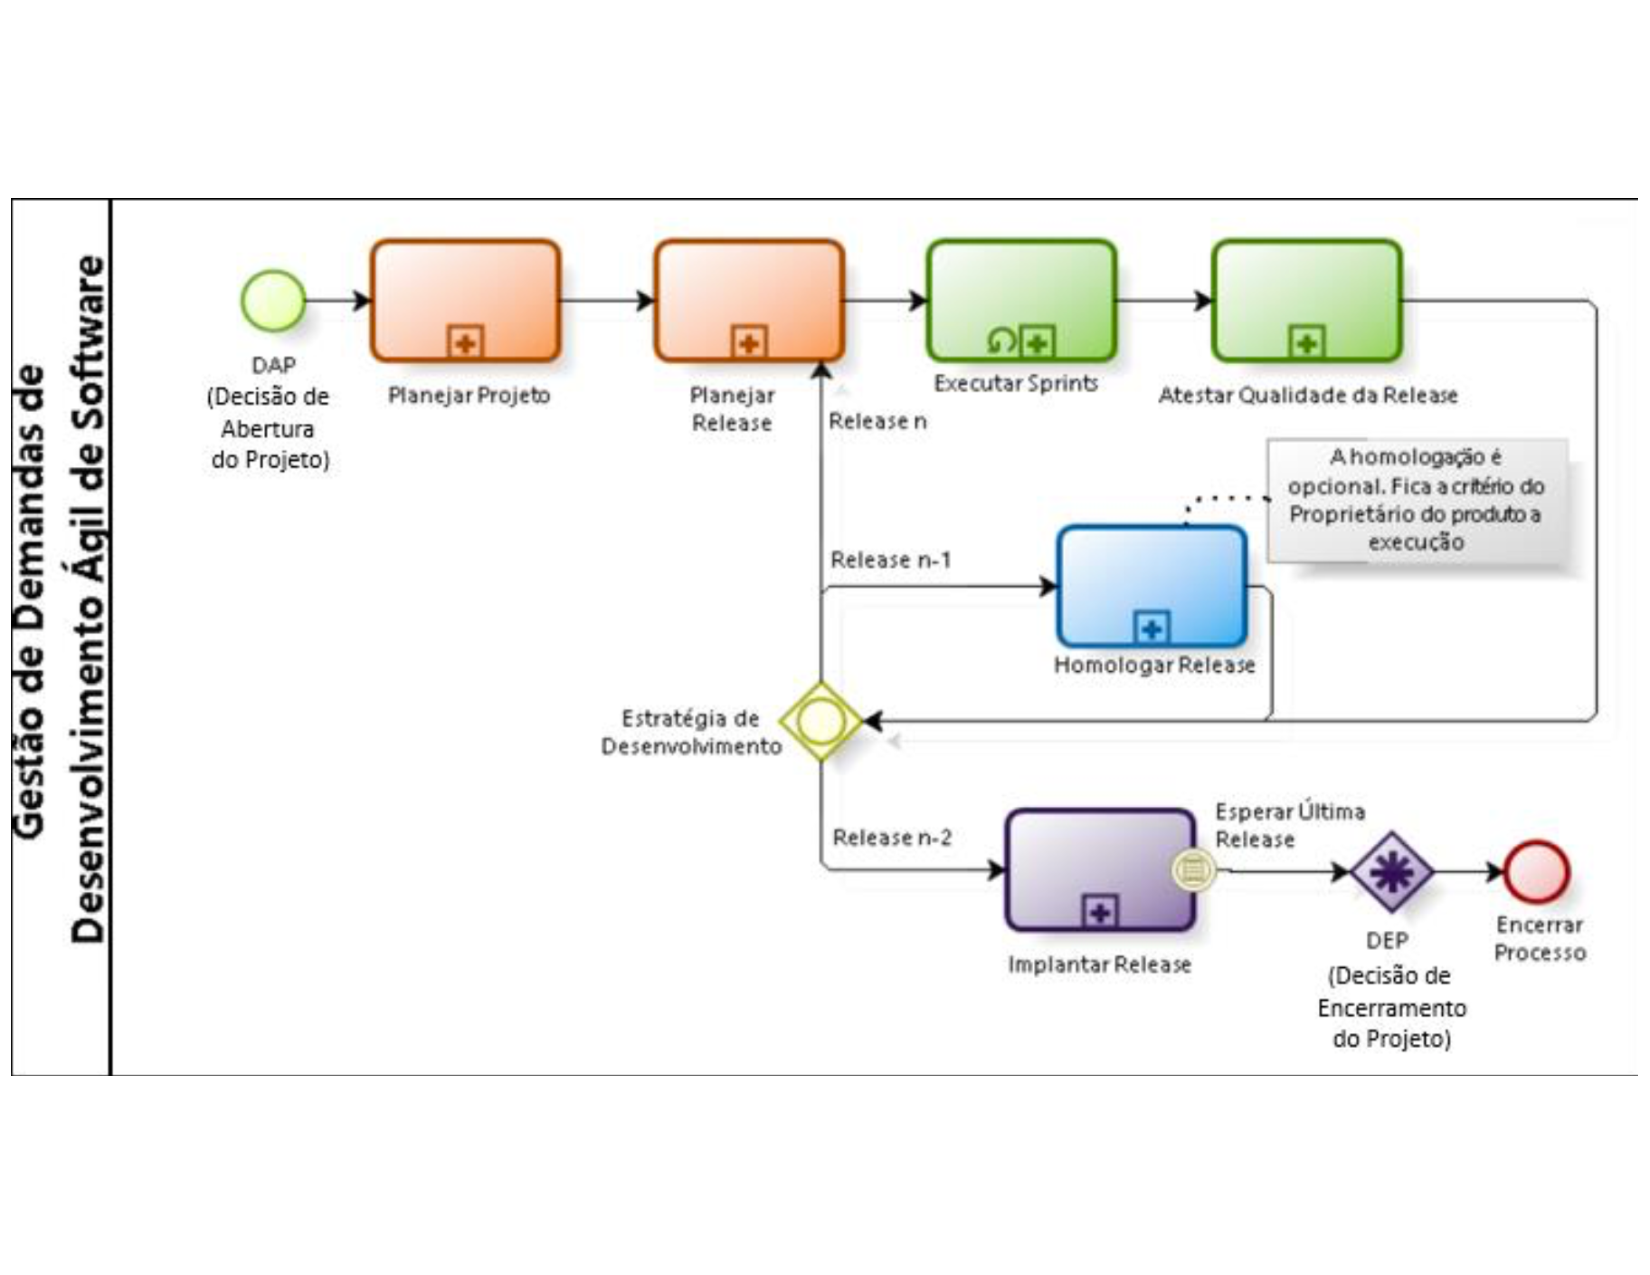
\includegraphics[scale=0.40]{Proc_des.pdf}
\caption{Processo de Desenvolvimento Adotado Pelo Órgão X. Fonte: \cite{luiza_yago}}
\label{img:proc_des}
\end{figure}




\graphicspath{{figuras/}}
\begin{figure}[h!]
\centering
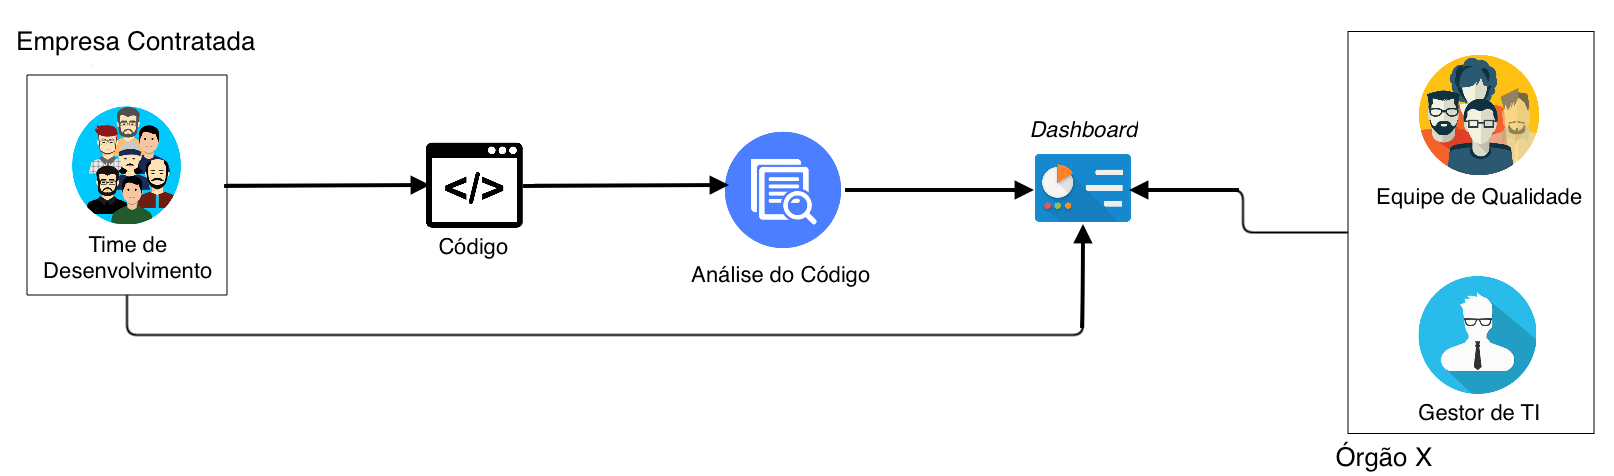
\includegraphics[scale=0.30]{proc_ver.png}
\caption{Ciclo de Verificação Utilizando a Solução Compartilhada Entre Órgão Contratante e Empresa Contratada}
\label{img:ciclo_ver}
\end{figure}


\section{Coleta das Métricas}
Para fazer a coleta das métricas, será utilizada a ferramenta SonarQube. Como já informado na capítulo de Suporte Tecnológico, esse suporte é muito utilizado em Órgãos Públicos e em editais por ser uma ferramenta \textit{open-source}. Nesse contexto, a coleta das métricas é feita de maneira dinamica, onde o que usuario decide qual suíte de metricas vai utilizar, podendo utilizar uma customizada ou utilizar uma como base. A presente proposta irá utilizar as suítes de métricas estabelecidas no edital do DNPM \cite{edital}). Portanto, serão utilizadas as suítes de métricas de Chidamber-Kemerer e a Suíte MOOD.

O \textit{dashboard} será customizável de acordo com a necessidade do Órgão. O Ógão poderá escolher quais métricas deseja usar e qual a faixa de valores aceitáveis para as métricas, caso ele queira. Será possível ainda, utilizar uma suíte de métricas já customizada e com valores definidos. 

As métricas "Violações do tipo Blocker", "Violações do tipo Major" e "Violações do tipo Minor" são estipuladas de acordo com o próprio perfil do Sonar, chamado Sonar Way. Contudo, a melhor maneira seria criar um perfil com as regras da própria organização garantindo uma avaliação mais focada no objetivo do Órgão.

O objetivo deste trabalho é criar uma ferramenta que auxilie na auditoria de produtos de software entregues por empresas tercerizadas. Entretanto percebe-se que ainda que o trabalho possua grande aprovação, dificilmente o mesmo irá substituir o fator humano da auditoria. Portanto, o software compreende apenas um suporte que visa facilitar a avaliação geral do software entregue sob o ponto de vista da qualidade de código. Recomenda-se, uma vez que o software seja submetido à ferramenta e seja aceito, a realização de uma auditoria em cima de uma amostragem do software entregue, sob o olhar de um analista especializado para tal atividade.

\section{Criação do \textit{Dashboard}}
Com as informações \textit{obtidas}, o dashboard funcionará como uma tela para visualização dessas métricas. A solução é composta por duas telas. Uma mostrando uma visão geral dos projetos, com indicadores quanto à aprovação ou reprovação de cada projeto seguindo os limites estabelecidos pelo edital \cite{edital}. A segunda tela consiste em uma visão mais detalhada sobre cada projeto, mostrando a evolução do projeto em cada métrica e com um \textit{link} para o Sonar de cada métrica para um aprofundamento.

\section{Avaliação}
A avaliação do \textit{dashboard} será feita por parte de um gestor de tecnologia de um Órgão Público. Ele avaliará aspectos de usabilidade da ferramenta e se a ferramenta possuiria condições mínimas de ser implantada. Caso não seja possível essa avaliação com um profissional da área, a avaliação será feita através de professores que possuem tal experiência com contratação de software para Órgãos Públicos, novamente avaliando aspectos como usabilidade e melhorias necessárias para implantação em um Órgão.
Para fazer esta avaliação, o gestor responderá a um questionário contendo, inicialmente, cinco perguntas, referentes ao uso e às funcionalidades do software produzido. Uma primeira verão do questionário consta na Figura \ref{img:questionario}

\graphicspath{{figuras/}}
\begin{figure}[h!]
\centering
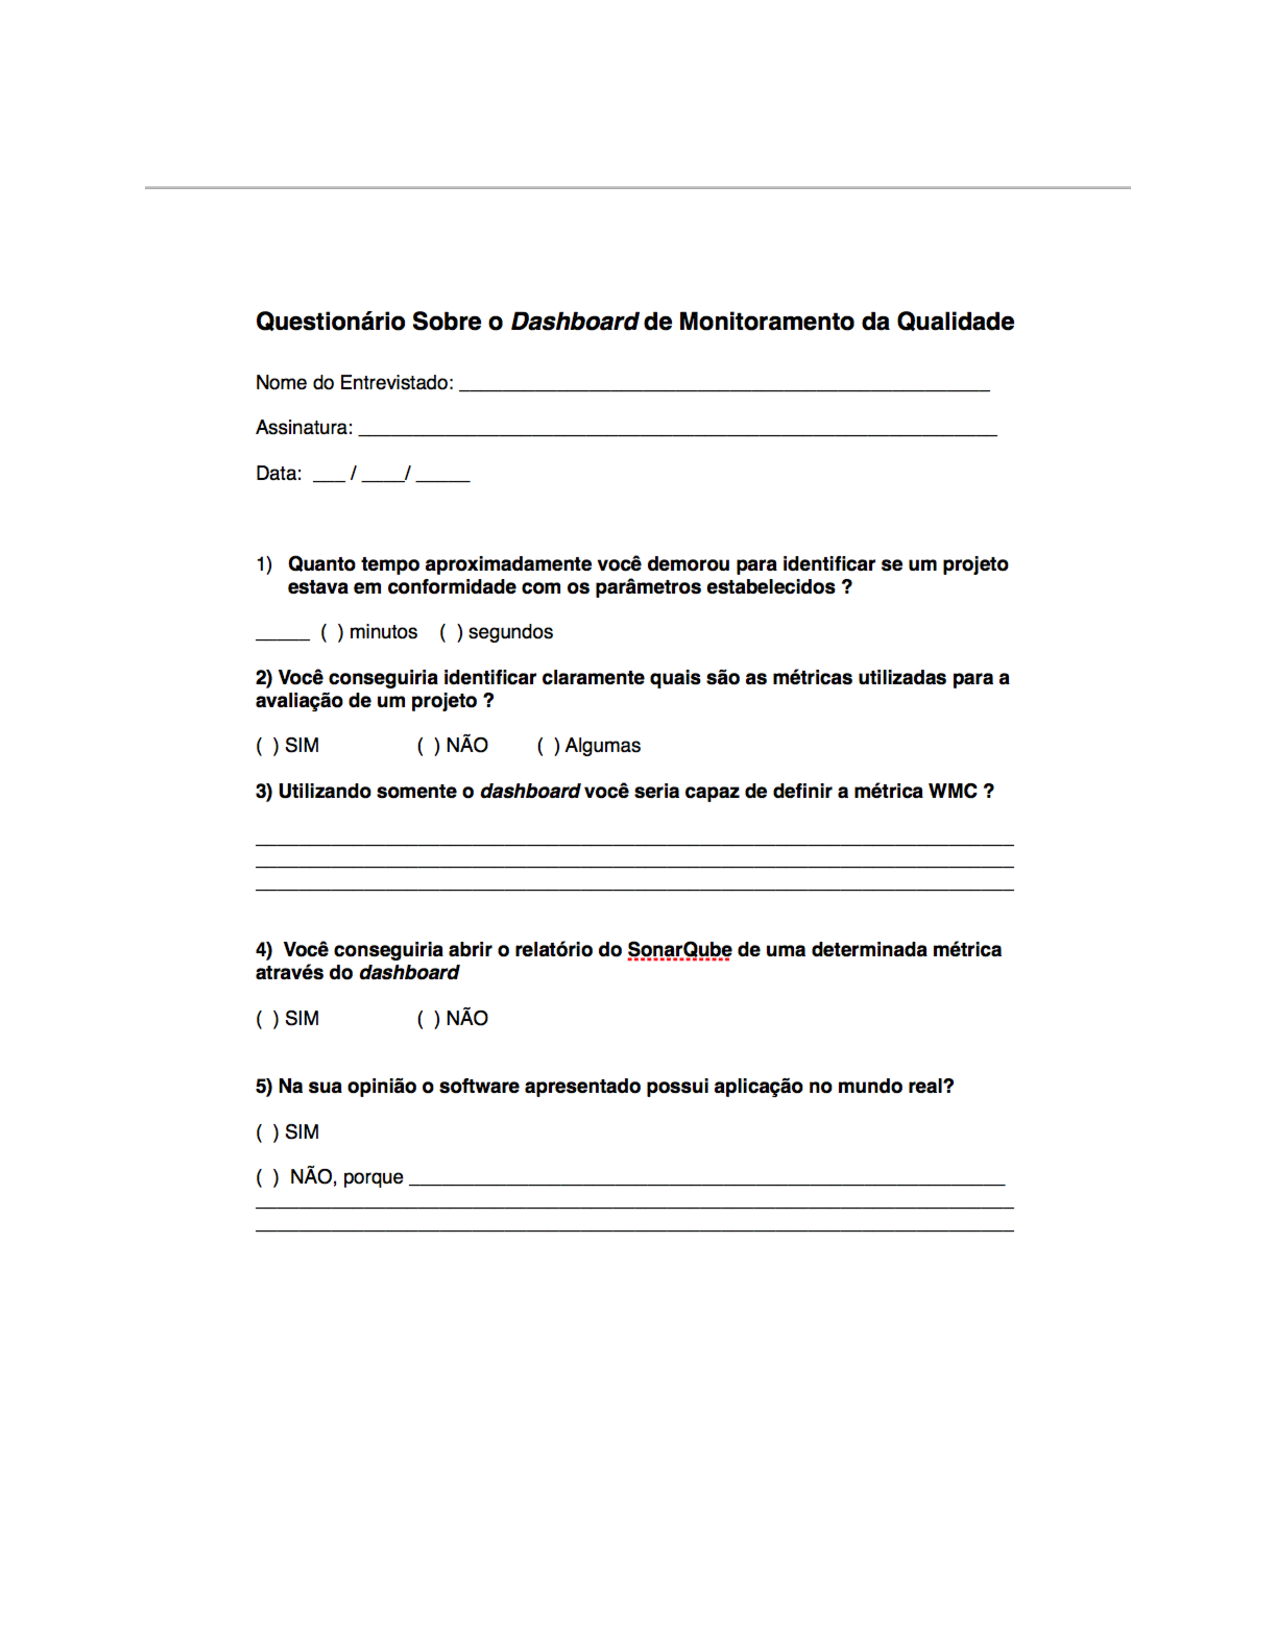
\includegraphics[scale=1.00]{questionario}
\caption{Questionário a ser aplicado ao fim do período de teste}
\label{img:questionario}
\end{figure}

\section{Resumo do Capítulo}
A proposta deste trabalho é criar uma maneira facilitada de acompanhar a qualidade de código estático dos produtos de software entregues pelas tercerizadas. Para fazer esta análise, a solução orienta-se por uma ferramenta de análise estática SonarQube e por um conjunto de métricas relacionadas às boas práticas de programação. A solução encontrada é a utilização de um \textit{dashboard} que mostre o real estado de um projeto, e que através de indicadores, seja possível determinar a qualidade do código. A última etapa deste trabalho consiste na avaliação do trabalho produzido, a qual será feita juntamente com um gestor de projeto de um Órgão Público ou um professor da insituição de ensino que responderá a um questionário quanto ao software produzido.